\section{\texorpdfstring{\Cref{chap:lifelong}}{} 的补充结果}

\subsection{偏差分析}

在本小节中，推导一个比 \Cref{lem:bias_bound} 中提供的界更紧但表达式更复杂的界。值得注意的是，该界对 $\omega=1$ 也成立。

\begin{lemma}
\label{lem:bias_general}
在 \Cref{ass:sce} 和 \Cref{ass:sch} 下，对于 $0<\omega\leq1$，估计器 $\widehat{J}_{T,\alpha,\beta}(\boldsymbol\rho)$ 的偏差可界定为：
\begin{align*}
    &\left\vert J_{T,\beta}(\boldsymbol\rho) - \mathbb{E}^{\boldsymbol\rho}_{T,\alpha}[\widehat{J}_{T,\alpha,\beta}] \right\vert
    \\
    &\qquad \le\left(L_{\mathcal{M}} + 2\maximumreward L_\nu\right) C_{\gamma}(\beta) \left(\omega
    \frac{1-\alpha\omega^{\alpha-1} + (\alpha-1) \omega^\alpha}{(1-\omega)(1-\omega^\alpha)} + \frac{1}{1-\gamma}\right),
\end{align*}
其中 $C_\gamma(\beta)$ 定义如 \Cref{eq:def_function_C}。
特别地，对于 $\omega=1$，该界是前式在 $\omega \rightarrow 1$ 时的极限，为：
\begin{align*}
    \left|J_{T,\beta}(\boldsymbol\rho) - \mathbb{E}^{\boldsymbol\rho}_{T,\alpha}[\widehat{J}_{T,\alpha,\beta}] \right|\le \left(L_{\mathcal{M}} + 2\maximumreward L_\nu\right) C_{\gamma}(\beta) \left(\frac{\alpha-1}{2} + \frac{1}{1-\gamma}  \right).
\end{align*}
\end{lemma}
\begin{proof}
回顾 $\widehat{J}_{T,\alpha,\beta}(\boldsymbol\rho)$ 的定义：
\begin{align*}
    \mathbb{E}^{\boldsymbol\rho}_{T,\alpha}\left[\widehat{J}_{T,\alpha,\beta}(\boldsymbol\rho)\right] & = \sum_{t=T-\alpha+1}^T \omega^{T-t}  \int_{\Theta} \nu_{\boldsymbol\rho}(\boldsymbol\theta|t) \frac{\sum_{s=T+1}^{T+\beta} \widehat{\gamma}^s \nu_{\boldsymbol\rho}(\boldsymbol\theta|s)}{\sum_{k=T-\alpha+1}^T \omega^{T-t} \nu_{\boldsymbol\rho}(\boldsymbol\theta|k)} \mathbb{E}_t^{\pi_{\boldsymbol\theta}}[r]  \de \boldsymbol\theta \\
    & = \sum_{s=T+1}^{T+\beta} \widehat{\gamma}^s \int_{\Theta}  \nu_{\boldsymbol\rho}(\boldsymbol\theta|s) \frac{\sum_{t=T-\alpha+1}^T \omega^{T-t} \nu_{\boldsymbol\rho}(\boldsymbol\theta|t) \mathbb{E}_t^{\pi_{\boldsymbol\theta}}[r]  }{\sum_{k=T-\alpha+1}^T \omega^{T-k} \nu_{\boldsymbol\rho}(\boldsymbol\theta|k)} \de \boldsymbol\theta.
\end{align*}
注意到 $J_{T,\beta}(\boldsymbol\rho) = \sum_{s=T+1}^{T+\beta} \widehat{\gamma}^s \int_{\Theta} \nu_{\boldsymbol\rho}(\boldsymbol\theta|s) \mathbb{E}_s^{\pi_{\boldsymbol\theta}}[r] \de \boldsymbol\theta$。
因此，
\begin{align*}
    &\left\vert \mathbb{E}^{\boldsymbol\rho}_{T,\alpha}\left[\widehat{J}_{T,\alpha,\beta}(\boldsymbol\rho)\right] - J_{T,\beta}(\boldsymbol\rho)\right\vert
    \\
    &\qquad =\left| \sum_{s=T+1}^{T+\beta} \widehat{\gamma}^s \int_{\Theta}  \nu_{\boldsymbol\rho}(\boldsymbol\theta|s) \frac{\sum_{t=T-\alpha+1}^T \omega^{T-t} \nu_{\boldsymbol\rho}(\boldsymbol\theta|t) \mathbb{E}_t^{\pi_{\boldsymbol\theta}}[r]  }{\sum_{k=T-\alpha+1}^T \omega^{T-k} \nu_{\boldsymbol\rho}(\boldsymbol\theta|k)} \de \boldsymbol\theta \right.
    \\
    &\qquad - \left.\sum_{s=T+1}^{T+\beta} \widehat{\gamma}^s \int_{\Theta} \nu_{\boldsymbol\rho}(\boldsymbol\theta|s) \mathbb{E}_s^{\pi_{\boldsymbol\theta}}[r] \de \boldsymbol\theta \right|
    \\
    &\qquad = \left| \sum_{s=T+1}^{T+\beta} \widehat{\gamma}^s \int_{\Theta}  \nu_{\boldsymbol\rho}(\boldsymbol\theta|s) \frac{\sum_{t=T-\alpha+1}^T \omega^{T-t} \nu_{\boldsymbol\rho}(\boldsymbol\theta|t) \left(\mathbb{E}_t^{\pi_{\boldsymbol\theta}}[r] - \mathbb{E}_s^{\pi_{\boldsymbol\theta}}[r] \right) }{\sum_{k=T-\alpha+1}^T \omega^{T-k} \nu_{\boldsymbol\rho}(\boldsymbol\theta|k)} \de \boldsymbol\theta  \right|.
\end{align*}
接下来，在上式最后一项中加入并移除量 $\textstyle\overline{\nu}(\boldsymbol\theta) \coloneq \frac{1}{C_{\omega}(\alpha)} \sum_{k=T-\alpha+1}^T \omega^{T-k} \nu_{\boldsymbol\rho}(\boldsymbol\theta|k)$，得到：
\begin{align*}
   &\Bigg| \sum_{s=T+1}^{T+\beta} \widehat{\gamma}^s \int_{\Theta}  \nu_{\boldsymbol\rho}(\boldsymbol\theta|s) \frac{\sum_{t=T-\alpha+1}^T \omega^{T-t} \nu_{\boldsymbol\rho}(\boldsymbol\theta|t) \left(\mathbb{E}_t^{\pi_{\boldsymbol\theta}}[r] - \mathbb{E}_s^{\pi_{\boldsymbol\theta}}[r] \right) }{\sum_{k=T-\alpha+1}^T \omega^{T-k} \nu_{\boldsymbol\rho}(\boldsymbol\theta|k)} \de \boldsymbol\theta  \Bigg|  \\
   &\qquad = \left| \sum_{s=T+1}^{T+\beta} \widehat{\gamma}^s \int_{\Theta}  \left(\nu_{\boldsymbol\rho}(\boldsymbol\theta|s) \pm \overline{\nu}_{\boldsymbol\rho}(\boldsymbol\theta)\right) \frac{\sum_{t=T-\alpha+1}^T \omega^{T-t} \nu_{\boldsymbol\rho}(\boldsymbol\theta|t)  \left(\mathbb{E}_t^{\pi_{\boldsymbol\theta}}[r] - \mathbb{E}_s^{\pi_{\boldsymbol\theta}}[r] \right) }{C_\omega(\alpha) \overline{\nu}(\boldsymbol\rho)} \de \boldsymbol\theta  \right|\\
   &\qquad \le \underbrace{\left| \sum_{s=T+1}^{T+\beta} \widehat{\gamma}^s \int_{\Theta}  \overline{\nu}_{\boldsymbol\rho}(\boldsymbol\theta)  \frac{\sum_{t=T-\alpha+1}^T \omega^{T-t} {\nu}_{\boldsymbol\rho}(\boldsymbol\theta|t) \left(\mathbb{E}_t^{\pi_{\boldsymbol\theta}}[r] - \mathbb{E}_s^{\pi_{\boldsymbol\theta}}[r] \right) }{C_\omega(\alpha) \overline{\nu}(\boldsymbol\rho)} \de \boldsymbol\theta  \right|}_{\text{(a)}} \\
   &\qquad \quad + \underbrace{\left| \sum_{s=T+1}^{T+\beta} \widehat{\gamma}^s \int_{\Theta}  \left(\nu_{\boldsymbol\rho}(\boldsymbol\theta|s) - \overline{\nu}_{\boldsymbol\rho}(\boldsymbol\theta)\right) \frac{\sum_{t=T-\alpha+1}^T \omega^{T-t} \nu_{\boldsymbol\rho}(\boldsymbol\theta|t) \left(\mathbb{E}_t^{\pi_{\boldsymbol\theta}}[r] - \mathbb{E}_s^{\pi_{\boldsymbol\theta}}[r] \right) }{C_\omega(\alpha) \overline{\nu}(\boldsymbol\rho)} \de \boldsymbol\theta  \right|}_{\text{(b)}}.
\end{align*}
可以对 (a) 进行如下界定，
\begin{align}
    \text{(a)} & = \frac{1}{C_\omega(\alpha)} \left| \sum_{s=T+1}^{T+\beta} \widehat{\gamma}^s \int_{\Theta}  \sum_{t=T-\alpha+1}^T \omega^{T-t} {\nu}_{\boldsymbol\rho}(\boldsymbol\theta|t) \left(\mathbb{E}_t^{\pi_{\boldsymbol\theta}}[r] - \mathbb{E}_s^{\pi_{\boldsymbol\theta}}[r] \right) \de \boldsymbol\theta  \right|
    \nonumber\\
    & \le \frac{1}{C_\omega(\alpha)}  \sum_{s=T+1}^{T+\beta} \widehat{\gamma}^s \int_{\Theta}  \sum_{t=T-\alpha+1}^T \omega^{T-t} {\nu}_{\boldsymbol\rho}(\boldsymbol\theta|t) \left|\mathbb{E}_t^{\pi_{\boldsymbol\theta}}[r] - \mathbb{E}_s^{\pi_{\boldsymbol\theta}}[r] \right| \de \boldsymbol\theta
    \nonumber\\
    &  \le \frac{L_{\mathcal{M}}}{C_\omega(\alpha)}  \sum_{s=T+1}^{T+\beta} \widehat{\gamma}^s  \sum_{t=T-\alpha+1}^T \omega^{T-t} \int_{\Theta} \nu_{\boldsymbol\rho}(\boldsymbol\theta|t) \left|t-s \right|  \de \boldsymbol\theta
    \label{eq:last_tkt1}\\
    & \le \frac{L_{\mathcal{M}}}{C_\omega(\alpha)}  {\sum_{s=T+1}^{T+\beta} \widehat{\gamma}^s   \sum_{t=T-\alpha+1}^T \omega^{T-t} \left|t-s \right|},
    \label{eq:last_tkt2}
\end{align}
其中在 \Cref{eq:last_tkt2} 中使用了 $\textstyle\int_{\Theta} {\nu}_{\boldsymbol\rho}(\boldsymbol\theta|t) \de \boldsymbol\theta = 1$ 的事实，在 \Cref{eq:last_tkt1} 中使用了 \Cref{ass:sce}。
接下来处理 (b)，
\begin{align}
    (b) & \le 2\maximumreward  \sum_{s=T+1}^{T+\beta} \widehat{\gamma}^s \int_{\Theta}  \left|\nu_{\boldsymbol\rho}(\boldsymbol\theta|s) - \overline{\nu}_{\boldsymbol\rho}(\boldsymbol\theta)\right| \frac{\sum_{t=T-\alpha+1}^T \omega^{T-t} \nu_{\boldsymbol\rho}(\boldsymbol\theta|t) }{C_\omega(\alpha) \overline{\nu}(\boldsymbol\rho)} \de \boldsymbol\theta
    \nonumber\\
    & = 2\maximumreward  \sum_{s=T+1}^{T+\beta} \widehat{\gamma}^s \int_{\Theta}  \left|\nu_{\boldsymbol\rho}(\boldsymbol\theta|s) - \overline{\nu}_{\boldsymbol\rho}(\boldsymbol\theta)\right|  \de \boldsymbol\theta
    \nonumber\\
    & \le 2\maximumreward  \sum_{s=T+1}^{T+\beta} \widehat{\gamma}^s  \frac{1}{C_{\omega}(\alpha)} \sum_{t=T-\alpha+1}^{T} \omega^{T-t} \int_{\Theta} \left|\nu_{\boldsymbol\rho}(\boldsymbol\theta|s) - \nu_{\boldsymbol\rho}(\boldsymbol\theta|t) \right|  \de \boldsymbol\theta
    \nonumber\\
    & \le  \frac{2\maximumreward  L_{\nu}}{C_{\omega}(\alpha)} \sum_{s=T+1}^{T+\beta} \widehat{\gamma}^s   \sum_{t=T-\alpha+1}^{T} \omega^{T-t} \left|t - s \right|,
    \label{eq:last_tkt3}
\end{align}
其中在 \Cref{eq:last_tkt3} 中使用了 \Cref{ass:sch}。
合并 (a) 和 (b) 得到：
\begin{align*}
    \left\vert J_{T,\beta}(\boldsymbol\rho) - \mathbb{E}^{\boldsymbol\rho}_{T,\alpha}[\widehat{J}_{T,\alpha,\beta}] \right\vert \le \frac{L_{\mathcal{M}} + 2\maximumreward L_\nu}{C_\omega(\alpha)} \sum_{s=T+1}^{T+\beta} \sum_{t=T-\alpha+1}^{T} \widehat{\gamma}^s    \omega^{T-t} (s-t).
\end{align*}
以下推导使用与 \cite[Lemma~3.4]{jagerman2019people} 类似的结构。
首先，令 $m = s-T$ 和 $n=T-t$，得到，
\begin{align}
    \frac{1}{C_\omega(\alpha)}\sum_{t=T-\alpha+1}^{T} \omega^{T-t} (s-t)
    &=  \frac{1}{C_\omega(\alpha)}\sum_{n=0}^{\alpha-1} \omega^{n} (m+n) \nonumber\\
    &= m + \frac{1}{C_\omega(\alpha)}
    \sum_{n=1}^{\alpha-1} \omega^{n} n.\label{eq:sum_m_n}
\end{align}
现在研究以下两种情况。\\
\noindent$\bullet\;$\textbf{情况 $\omega<1$。}\indent 有，
\begin{align*}
    \frac{1}{C_\omega(\alpha)}\sum_{t=T-\alpha+1}^{T} \omega^{T-t} (s-t)
    &= m + \frac{1}{C_\omega(\alpha)} \omega \frac{d}{d\omega}
    \sum_{n=1}^{\alpha-1} \omega^{n}
    \\
    &= m + \frac{1}{C_\omega(\alpha)} \omega
    \frac{1-\alpha\omega^{\alpha-1} + (\alpha-1) \omega^\alpha}{(1-\omega)^2}
    \\
    &= m + \omega
    \frac{1-\alpha\omega^{\alpha-1} + (\alpha-1) \omega^\alpha}{(1-\omega)(1-\omega^\alpha)},
\end{align*}
这给出，
\begin{align*}
    &\left|J_{T,\beta}(\boldsymbol\rho) - \mathbb{E}^{\boldsymbol\rho}_{T,\alpha}\left[\widehat{J}_{T,\alpha,\beta}\right] \right|
    \\
    &\qquad \le \frac{L_{\mathcal{M}} + 2\maximumreward L_\nu}{C_\omega(\alpha)} \sum_{s=T+1}^{T+\beta} \sum_{t=T-\alpha+1}^{T} \widehat{\gamma}^s    \omega^{T-t} (s-t)
    \\
    &\qquad= \left(L_{\mathcal{M}} + 2\maximumreward L_\nu\right) \sum_{s=T+1}^{T+\beta} \widehat{\gamma}^s \left(m + \omega
    \frac{1-\alpha\omega^{\alpha-1} + (\alpha-1) \omega^\alpha}{(1-\omega)(1-\omega^\alpha)}\right)
    \\
    &\qquad= \left(L_{\mathcal{M}} + 2\maximumreward L_\nu\right) \sum_{s=T+1}^{T+\beta} \widehat{\gamma}^s \left((s-T) + \omega
    \frac{1-\alpha\omega^{\alpha-1} + (\alpha-1) \omega^\alpha}{(1-\omega)(1-\omega^\alpha)}\right)
    \\
    &\qquad= \left(L_{\mathcal{M}} + 2\maximumreward L_\nu\right)  \left(\frac{1-\gamma^\beta}{1-\gamma}  \omega
    \frac{1-\alpha\omega^{\alpha-1} + (\alpha-1) \omega^\alpha}{(1-\omega)(1-\omega^\alpha)} + \sum_{k=0}^{\beta-1} \gamma^k (k+1)\right)
    \\
    &\qquad= \left(L_{\mathcal{M}} + 2\maximumreward L_\nu\right)  \left(\frac{1-\gamma^\beta}{1-\gamma}  \omega
    \frac{1-\alpha\omega^{\alpha-1} + (\alpha-1) \omega^\alpha}{(1-\omega)(1-\omega^\alpha)} + \frac{1-\gamma^\beta}{(1-\gamma)^2}\right)
    \\
    &\qquad= \left(L_{\mathcal{M}} + 2\maximumreward L_\nu\right) \frac{1-\gamma^\beta}{1-\gamma} \left(\omega
    \frac{1-\alpha\omega^{\alpha-1} + (\alpha-1) \omega^\alpha}{(1-\omega)(1-\omega^\alpha)} + \frac{1}{1-\gamma}\right).
\end{align*}
\noindent$\bullet\;$\textbf{情况 $\omega=1$。}\indent 此时，\Cref{eq:sum_m_n} 变为：
\begin{align*}
    \frac{1}{C_\omega(\alpha)}\sum_{t=T-\alpha+1}^{T} \omega^{T-t} (s-t)
     = m + \frac{1}{\alpha}
    \sum_{n=1}^{\alpha-1} n = m + \frac{\alpha-1}{2}.
\end{align*}
因此，界变为：
\begin{align*}
    \left|J_{T,\beta}(\boldsymbol\rho) - \mathbb{E}^{\boldsymbol\rho}_{T,\alpha}\left[\widehat{J}_{T,\alpha,\beta}\right] \right|
    &\leq \left(L_{\mathcal{M}} + 2\maximumreward L_\nu\right) \sum_{s=T+1}^{T+\beta} \widehat{\gamma}^s \left(m +  \frac{\alpha-1}{2}\right)
    \\
    &= \left(L_{\mathcal{M}} + 2\maximumreward L_\nu\right) \left(C_{\gamma}(\beta)  \frac{\alpha-1}{2} + \sum_{k=0}^{\beta-1}\gamma^k (k+1)  \right)
    \\
    &= \left(L_{\mathcal{M}} + 2\maximumreward L_\nu\right) C_{\gamma}(\beta) \left(\frac{\alpha-1}{2} + \frac{1}{1-\gamma}  \right).
\end{align*}
\end{proof}




\subsection{关于混合分布之间 \Renyi 散度的变分界}
\label{app:var_bound}
在本附录中，讨论混合分布 $\textstyle\Psi = \sum_{i=1}^L \zeta_i P_i$ 和 $\textstyle\Phi = \sum_{j=1}^K \mu_j Q_j$ 之间的 \Renyi 散度 $\exponentialrenyidivergence[\alpha](\Psi\left\Vert\Phi\right.)$ 的若干上界，其中 $\forall i \in [\![1,L]\!],\ j \in [\![1,K]\!],\  0<\zeta_i,\ \mu_j <1$ 且 $\textstyle\sum_{i=1}^L \zeta_i = \sum_{j=1}^K \mu_j= 1$。我们限制在 $\alpha\ge1$ 的情况。首先，报告 \cite{papini2019optimistic} 中的一个基本结果。

\begin{lemma}[Lemma~4, \cite{papini2019optimistic}]
\label{pp:papini_lemma}
    考虑变分参数集 $\{\psi_{ij}\}_{(i,j)\in[\![1,L]\!]\times [\![1,K]\!]}$ 和 $\{\phi_{ij}\}_{(i,j)\in[\![1,L]\!]\times [\![1,K]\!]}$，
    满足 $\phi_{ij},\psi_{ij}\ge 0$，$\textstyle\sum_{i=1}^L \psi_{ij} = \mu_j$ 且 $\textstyle\sum_{j=1}^K \phi_{ij} = \zeta_i$。
    则对于任何 $\alpha\ge 1$ 以及上述定义的混合分布，有：
    \begin{align}
    \label{eq:papini_lemma}
        \exponentialrenyidivergence[\alpha](\Psi\left\Vert\Phi\right.) \leq \sum_{i=1}^L\sum_{j=1}^K \phi_{ij}^{\alpha} \psi_{ij}^{1-\alpha} \exponentialrenyidivergence[\alpha](P_i\left\Vert Q_j\right)^{\alpha-1}.
    \end{align}
\end{lemma}

寻找最紧的上界相当于找到使 \Cref{eq:papini_lemma} 最小化的 $\{\psi_{ij}\}$ 和 $\{\phi_{ij}\}$ 的值。一个直接但不成功的选择是均匀值。下面，我们推导六种替代方法用于选择 $\{\psi_{ij}\}$ 和 $\{\phi_{ij}\}$，以获得更紧的界。最后，在一个玩具问题上比较这些可能的界，以选择最佳的一个。



\subsubsection{直接凸优化}
在各自的约束下，最小化 \Cref{eq:papini_lemma}（其中 $\phi_{ij}\geq 0$ 和 $\psi_{ij}\geq 0$）的问题是凸的。因此，可以采用相当直接的方法，使用梯度下降法来优化这些变分参数。

\textbf{带重置。}
第一种方法是先从变分参数的均匀分布开始，然后连续多步沿着梯度方向更新。每当 POLIS 需要对 \Renyi 散度进行界定时，都需要应用相同的过程。我们将此方法称为\emph{带重置的直接优化}。

\textbf{无重置。}
第二个想法也是连续多步沿着梯度方向更新，但从先前变分参数的值而非均匀分布开始。更具体地说，每次 POLIS 需要对 \Renyi 散度进行界定时，前一次界的变分参数被用作新优化问题的起点。我们将此方法称为\emph{无重置的直接优化}。


\subsubsection{两步最小化}
每次需要上界时都必须求解优化问题，这并不令人满意。在本节中，提出基于以下定理的替代推导。

\begin{thm}[Theorem~5, \cite{papini2019optimistic}]
\label{th:mix_phi}
    考虑概率分布 $P$ 和之前的混合分布 $\Phi$，则对于任何 $\alpha\geq1$，有：
    \begin{align*}
        \exponentialrenyidivergence[\alpha](P\left\Vert\Phi\right.) \leq     \frac{1}{\sum_{j=1}^K\frac{\mu_j}{\exponentialrenyidivergence[\alpha]( P \Vert Q_j)}}.
    \end{align*}
\end{thm}

注意该界涉及 $P$ 与混合分量之间 \Renyi 散度的调和均值。
类似地，为 $\exponentialrenyidivergence[\alpha](\Psi\left\Vert Q\right)$ 推导一个界，其中 $\Psi$ 是混合分布。

\begin{prop}
\label{pp:mix_psi}
    设 $Q$ 为一个概率测度，考虑之前的混合分布 $\Psi$，则对于任何 $\alpha\geq1$，有：
    \begin{align*}
        \exponentialrenyidivergence[\alpha](\Psi\left\Vert Q\right.) \leq \left(\sum_{i=1}^L \zeta_i \exponentialrenyidivergence[\alpha](P_i\Vert Q)^{\frac{\alpha-1}{\alpha}}\right)^{\frac{\alpha}{\alpha-1}}.
    \end{align*}
\end{prop}
\begin{proof}
    根据 \cite{papini2019optimistic}，由于 \Cref{eq:papini_lemma} 关于 $\{\psi_i\}$ 是凸的，可以使用拉格朗日乘子法找到 $\{\psi_i\}$ 的最优值，
    \begin{align*}
        \psi_i = \frac{\zeta_i \exponentialrenyidivergence[\alpha](P_i \Vert Q)^{\frac{\alpha-1}{\alpha}}}{\sum_{i=1}^L \zeta_i \exponentialrenyidivergence[\alpha](P_i\Vert Q)^{\frac{\alpha-1}{\alpha}}}.
    \end{align*}
    将该值代入原问题得到，
    \begin{align*}
        \exponentialrenyidivergence[\alpha](\Psi\left\Vert Q\right.)^{\alpha-1}
        &\leq \sum_{i=1}^L \zeta_i^\alpha \left(\frac{\zeta_i \exponentialrenyidivergence[\alpha](P_i \Vert Q)^{\frac{\alpha-1}{\alpha}}}{\sum_{i=1}^L \zeta_i \exponentialrenyidivergence[\alpha](P_l\Vert Q)^{\frac{\alpha-1}{\alpha}}} \right)^{1-\alpha} \exponentialrenyidivergence[\alpha](P_i \Vert Q)^{\alpha-1}
        \\
        &= \sum_{i=1}^L \zeta_i\frac{ \exponentialrenyidivergence[\alpha](P_i \Vert Q)^{(1-\alpha)\frac{\alpha-1}{\alpha} +\alpha-1}}{\left(\sum_{l=1}^L \zeta_l \exponentialrenyidivergence[\alpha](P_l\Vert Q)^{\frac{\alpha-1}{\alpha}}\right)^{1-\alpha}}
        \\
        &= \frac{\sum_{i=1}^L \zeta_i \exponentialrenyidivergence[\alpha](P_i \Vert Q)^{\frac{\alpha-1}{\alpha} }}{\left(\sum_{i=1}^L \zeta_i \exponentialrenyidivergence[\alpha](P_i\Vert Q)^{\frac{\alpha-1}{\alpha}}\right)^{1-\alpha}}
        \\
        &= \left(\sum_{i=1}^L \zeta_i \exponentialrenyidivergence[\alpha](P_i\Vert Q)^{\frac{\alpha-1}{\alpha}}\right)^{\alpha}.
    \end{align*}
\end{proof}

特别地，与 \Cref{th:mix_phi} 相比，该界现在涉及 $Q$ 与混合元素之间 \Renyi 散度的指数 $\textstyle\frac{\alpha-1}{\alpha}$ 的加权幂均值。
现在，可以组合 \Cref{th:mix_phi} 和 \Cref{pp:mix_psi} 来寻找 $\exponentialrenyidivergence[\alpha](\Psi\left\Vert\Phi\right)$ 的界。
根据先应用哪个结果，得到不同的界。


\textbf{两步 $\psi$ 优先。}
\label{subsubsec:two_steps_psi_first}
先应用 \Cref{pp:mix_psi} 再应用 \Cref{th:mix_phi} 得到以下界，我们称之为\textit{两步 $\psi$ 优先}。

\begin{prop}
\label{pp:var_bound_2_steps_psi_first}
    在 \Cref{pp:papini_lemma} 的假设下，有：
    \begin{align*}
        \exponentialrenyidivergence[\alpha](\Psi\left\Vert \Phi\right.)
        &\leq
        \left(\sum_{i=1}^L \zeta_i \exponentialrenyidivergence[\alpha](P_i\Vert \Psi)^{\frac{\alpha-1}{\alpha}}\right)^{\frac{\alpha}{\alpha-1}}\\
        &\leq
        \left(\sum_{i=1}^L \zeta_i \frac{1}{\left(\sum_{j=1}^K\frac{\mu_j}{\exponentialrenyidivergence[\alpha]( P_i \Vert Q_j)}\right)^{\frac{\alpha-1}{\alpha}}}\right)^{\frac{\alpha}{\alpha-1}}.
    \end{align*}
\end{prop}


\renyidivergencebound*
\begin{proof}
    结果通过将 $\alpha=2$ 的 \Cref{pp:var_bound_2_steps_psi_first} 应用于混合分布 $\textstyle\sum_{s=T+1}^{T+\beta} \frac{\widehat{\gamma}^s}{C_\gamma(\beta)} \nu_{\boldsymbol\rho}(\cdot|s)$ 和 $\textstyle\sum_{t=T-\alpha+1}^{T} \frac{\omega^{T-t} }{C_\omega(\alpha)}\nu_{\boldsymbol\rho}(\cdot|t)$ 得到。
\end{proof}



\textbf{两步 $\phi$ 优先。}
另一种方式，先应用 \Cref{th:mix_phi} 再应用 \Cref{pp:mix_psi} 得到以下界，称之为\textit{两步 $\phi$ 优先}。

\begin{prop}
    在 \cref{pp:papini_lemma} 的假设下，
    \begin{align*}
    \exponentialrenyidivergence[\alpha](\Psi\left\Vert \Phi\right.)
    &\leq \frac{1}{\sum_{j=1}^K \frac{\mu_j}{\exponentialrenyidivergence[\alpha](\Psi\Vert Q_j)}}
    \\
    &\leq \frac{1}{\sum_{j=1}^K \mu_j \left(\sum_{i=1}^L \zeta_i \exponentialrenyidivergence[\alpha](P_i\Vert Q_j)^{\frac{\alpha-1}{\alpha}}\right)^{-\frac{\alpha}{\alpha-1}} }.
\end{align*}
\end{prop}

将此结果应用于 \Cref{lem:variance_bound} 得到以下结果。

\begin{prop}[使用 {两步 $\phi$ 优先} 的下界]
    对于 $\delta>0$，以至少 $1-\delta$ 的概率，有
\begin{align*}
    &\mathbb{E}\left[\overline{J}_{T,\alpha,\beta} \right]
    \\
    &\qquad\geq
    \overline{J}_{T,\alpha,\beta} - \sqrt{
            \frac{1-\delta}{\delta} 2\maximumreward}
    \\
    &\qquad\cdot\sqrt{C_\gamma(\alpha)^2 +
            \frac{ C_\omega(\alpha)}{\sum_{ k=T-\alpha+1}^{ T}\omega^{T-k} \left(\sum_{ s=T+1}^{ T+\beta} \widehat{\gamma}^s d_2(\nu_{\boldsymbol\rho}(\cdot\vert s)\Vert \nu_{\boldsymbol\rho}(\cdot\vert k))^{\frac{1}{2}}\right)^{-2} }}.
\end{align*}
\end{prop}


\subsubsection{一步后均匀化}
在本节中，探索将一组变分参数表示为另一组的函数，然后再将其值代入 \Cref{eq:papini_lemma} 的可能性。在下一个命题中，给出 $\{\psi_{ij}\}_{(i,j)\in[\![1,L]\!]\times [\![1,K]\!]}$ 关于 $\{\phi_{ij}\}_{(i,j)\in[\![1,L]\!]\times [\![1,K]\!]}$ 的表达式，反之亦然。

\begin{prop}
    在与 \Cref{pp:papini_lemma} 相同的假设下，$\psi_{ij}$ 的最优值为
    \begin{align}
    \label{eq:psi_optim}
        \psi_{ij} = \mu_{j} \frac{\phi_{ij}\exponentialrenyidivergence[\alpha](P_i\Vert Q_j)^{\frac{\alpha-1}{\alpha}}}{\sum_{l=1}^L \phi_{lj}\exponentialrenyidivergence[\alpha](P_l\Vert Q_j)^{\frac{\alpha-1}{\alpha}}};
    \end{align}
    $\phi_{ij}$ 的最优值为
    \begin{align}
    \label{eq:phi_optim}
        \phi_{ij} = \frac{\zeta_i \psi_{ij}}{ \exponentialrenyidivergence[\alpha](P_i\Vert Q_j)} \left(\sum_{k=1}^K\frac{\psi_{ik}}{\exponentialrenyidivergence[\alpha](P_i\Vert Q_k)}\right)^{-1}.
    \end{align}
\end{prop}
\begin{proof}
    由 \Cref{eq:papini_lemma} 可知，
    \begin{align*}
        \exponentialrenyidivergence[\alpha](\Psi\Vert\Phi)^{\alpha-1}\leq\sum_{i=1}^{L}\sum_{j=1}^K \phi_{ij}^\alpha \psi_{ij}^{1-\alpha} \exponentialrenyidivergence[\alpha](P_i\Vert Q_j)^{\alpha-1}.
    \end{align*}
    该问题的拉格朗日函数为：
    \begin{align*}
        \mathcal{L}(\phi_{ij},\phi_{ij},\lambda_i^{\zeta},\lambda_j^{\mu})=\sum_{i=1}^{L}\sum_{j=1}^K \phi_{ij}^\alpha \psi_{ij}^{1-\alpha} \exponentialrenyidivergence[\alpha](P_i\Vert Q_j)^{\alpha-1} - \sum_{i=1}^L \lambda_i^{\zeta} (\sum_{j=1}^K \phi_{ij} - \zeta_i)
        - \sum_{j=1}^K \lambda_j^{\mu} (\sum_{i=1}^L \psi_{ij} - \mu_j).
    \end{align*}
    对变分变量求导并令其为零得到，
    \begin{align*}
        \frac{\partial \mathcal{L}}{\partial \phi_{ij}} &= \alpha \phi_{ij}^{\alpha-1} \psi_{ij}^{1-\alpha} \exponentialrenyidivergence[\alpha] (P_i\Vert Q_j)^{\alpha-1}-\lambda_i^{\zeta} =0.
    \end{align*}
    这意味着：
    \begin{align*}
        \phi_{ij} = \frac{{\lambda_i^{\zeta}}^{\frac{1}{\alpha-1}}\psi_{ij}}{\alpha^{\frac{1}{\alpha-1}} \exponentialrenyidivergence[\alpha](P_i\Vert Q_j)}.
    \end{align*}
    回顾 $\sum_{j}\phi_{ij}=\zeta_i$，所以：
    \begin{align*}
        \left(\frac{{\lambda_i^{\zeta}}}{\alpha}\right)^{\frac{1}{\alpha-1}} \sum_{k=1}^K \frac{\psi_{ik}}{\exponentialrenyidivergence[\alpha](P_i\Vert Q_k)} = \zeta_l.
    \end{align*}
    这给出了 $\lambda_i^{\zeta}$ 的值：
    \begin{align*}
        \lambda_i^{\zeta} = \frac{\alpha \zeta_i^{\alpha-1}}{\left(\sum_{k=1}^K\frac{\psi_ik}{\exponentialrenyidivergence[\alpha](P_i\Vert Q_k)}\right)^{\alpha-1}}.
    \end{align*}
    最后，代入得到，
    \begin{align*}
        \phi_{ij} = \frac{\zeta_i \psi_{ij}}{ \exponentialrenyidivergence[\alpha](P_i\Vert Q_j)} \left(\sum_{k=1}^K\frac{\psi_{ik}}{\exponentialrenyidivergence[\alpha](P_i\Vert Q_k)}\right)^{-1}.
    \end{align*}
    对 $\psi_{ij}$ 做相同处理：
    \begin{align*}
        \frac{\partial \mathcal{L}}{\partial \psi_{ij}} &= (1-\alpha) \psi_{ij}^{\alpha} \psi_{ij}^{-\alpha} \exponentialrenyidivergence[\alpha] (P_i\Vert Q_j)^{\alpha-1}-\lambda_j^{\mu} = 0.
    \end{align*}
    这意味着
    \begin{align*}
        \psi_{ij} = \left(\frac{1-\alpha}{\lambda_j^{\mu}}\right)^{\frac{1}{\alpha}}\phi_{ij}\exponentialrenyidivergence[\alpha](P_i\Vert Q_j)^{\frac{\alpha-1}{\alpha}}.
    \end{align*}
    回顾 $\sum_{i}\psi_{ij}=\beta_j$，所以：
    \begin{align*}
        \left(\frac{1-\alpha}{\lambda_j^{\mu}}\right)^{\frac{1}{\alpha}} \sum_{l=1}^L \phi_{lj}\exponentialrenyidivergence[\alpha](P_l\Vert Q_j)^{\frac{\alpha-1}{\alpha}} = \mu_l.
    \end{align*}
    这给出了 $\lambda_j^{\beta}$ 的值：
    \begin{align*}
        \lambda_j^{\beta} = \frac{1-\alpha}{\mu_j^\alpha}\left(\sum_{l=1}^L \phi_{lj}\exponentialrenyidivergence[\alpha](P_l\Vert Q_j)^{\frac{\alpha-1}{\alpha}}\right)^\alpha .
    \end{align*}
    最后，代入得到，
    \begin{align*}
        \psi_{ij} = \mu_j \frac{\phi_{ij}\exponentialrenyidivergence[\alpha](P_i\Vert Q_j)^{\frac{\alpha-1}{\alpha}}}{\sum_{l=1}^L \phi_{lj}\exponentialrenyidivergence[\alpha](P_l\Vert Q_j)^{\frac{\alpha-1}{\alpha}}}.
    \end{align*}
\end{proof}


\textbf{均匀 $\psi$。}
在本节中，通过利用 \Cref{eq:phi_optim} 中 $\phi_{ij}$ 的最优值并将其代入 \Cref{eq:papini_lemma}，提出 \Cref{eq:papini_lemma} 的一个上界。然后将参数 $\psi_{ij}$ 设置为均匀值。
该界如下所示，称为\textit{均匀 $\psi$}。

\begin{prop}
在 \Cref{pp:papini_lemma} 的假设下，有
    \begin{align*}
        \exponentialrenyidivergence[\alpha](\Psi\vert\Phi)
        &\leq \sum_{i=1}^L \frac{\zeta_i^\alpha}{L^{1-\alpha}}
        \left(
            \sum_{j=1}^K \frac{\mu_j}{\exponentialrenyidivergence[\alpha](P_i \Vert Q_j)}
        \right)^{1-\alpha}.
    \end{align*}
\end{prop}
\begin{proof}
    将 \Cref{eq:phi_optim} 代入 \Cref{eq:papini_lemma} 得到，
    \begin{align*}
        \exponentialrenyidivergence[\alpha](\Psi\vert\Phi)
        &\leq \sum_{i=1}^L\sum_{j=1}^K \zeta_i^\alpha \frac{\psi_{ij}}{\exponentialrenyidivergence[\alpha](P_i \Vert Q_j)}
        \left(
            \sum_{k=1}^K \frac{\psi_{ik}}{\exponentialrenyidivergence[\alpha](P_i \Vert Q_k)}
        \right)^{-\alpha}
        \\
        &= \sum_{i=1}^L \zeta_i^\alpha
        \left(
            \sum_{j=1}^K \frac{\psi_{ij}}{\exponentialrenyidivergence[\alpha](P_i \Vert Q_j)}
        \right)^{1-\alpha}.
    \end{align*}
    然后，回顾约束 $\psi_{ij}\geq 0$ 和 $\textstyle\sum_{i=1}^L \psi_{ij}=\mu_j$，设置 $\psi_{ij}=\frac{\mu_j}{L}$ 满足这些约束并得到结果。
\end{proof}

与之前的界一样，将此结果应用于 \Cref{lem:variance_bound} 得到以下结果。

\begin{prop}[使用 {均匀 $\psi$} 的下界]
    对于 $\delta>0$，以至少 $1-\delta$ 的概率，有
    \begin{align*}
        &\mathbb{E}\left[\overline{J}_{T,\alpha,\beta} \right]
        \\
        &\qquad \geq  \overline{J}_{T,\alpha,\beta} -
        \sqrt{
            \frac{1-\delta}{\delta} 2  \maximumreward  }
        \\
        &\qquad
        \sqrt{
            C_\gamma(\alpha)^2 +
            \beta C_\omega(\alpha)
            \sum_{s=T+1}^{T+\beta} \widehat{\gamma}^{2s}
            \left(
                \sum_{k=T-\alpha+1}^T\frac{\omega^{T-k}}{ d_2(\nu_{\boldsymbol\rho}(\cdot\vert s)\Vert \nu_{\boldsymbol\rho}(\cdot\vert k))}
            \right)^{-1}.
        }
    \end{align*}
\end{prop}


\textbf{均匀 $\phi$。}

与之前的界类似，利用 \Cref{eq:phi_optim} 中 $\psi_{ij}$ 的最优值并将其代入 \Cref{eq:papini_lemma}。然后将参数 $\phi_{ij}$ 设置为均匀值。
该界如下所示，称为\textit{均匀 $\phi$}。

\begin{prop}
在 \Cref{pp:papini_lemma} 的假设下，有
    \begin{align*}
        \exponentialrenyidivergence[\alpha](\Psi\vert\Phi)
        &\leq \sum_{j=1}^K \frac{\mu_j^{1-\alpha}}{K^{\alpha}}  \left(\sum_{i=1}^L \zeta_i \exponentialrenyidivergence[\alpha](P_i \Vert Q_j)^{\frac{\alpha-1}{\alpha}}
        \right)^{\alpha}.
    \end{align*}
\end{prop}
\begin{proof}
    将 \Cref{eq:phi_optim} 代入 \Cref{eq:papini_lemma} 得到，
    \begin{align*}
        \exponentialrenyidivergence[\alpha](\Psi\vert\Phi)
        &\leq \sum_{i=1}^L\sum_{j=1}^K \mu_j^{1-\alpha} \frac{\phi_{ij}\exponentialrenyidivergence[\alpha](P_i \Vert Q_j)^{\frac{\alpha-1}{\alpha}}}{\left(\sum_{l=1}^L \phi_{lj}\exponentialrenyidivergence[\alpha](P_l \Vert Q_j)^{\frac{\alpha-1}{\alpha}}\right)^{1-\alpha}}
        \\
        &= \sum_{j=1}^K \mu_j^{1-\alpha} \left(\sum_{i=1}^L \phi_{ij}\exponentialrenyidivergence[\alpha](P_i \Vert Q_j)^{\frac{\alpha-1}{\alpha}}
        \right)^{\alpha}.
    \end{align*}
    然后，回顾约束 $\phi_{ij}\geq 0$ 和 $\textstyle\sum_{j=1}^K \phi_{ij}=\zeta_i$，设置 $\textstyle\phi_{ij}=\frac{\zeta_i}{K}$ 满足这些约束并得到结果。
\end{proof}

与之前的界一样，将此结果应用于 \Cref{lem:variance_bound} 得到以下结果。

\begin{prop}[使用 {均匀 $\phi$} 的下界]
    对于 $\delta>0$，以至少 $1-\delta$ 的概率，有
    \begin{align*}
        \mathbb{E}\left[\overline{J}_{T,\alpha,\beta} \right]
        &\geq  \overline{J}_{T,\alpha,\beta} -
        \sqrt{
            \frac{1-\delta}{\delta} 2 \maximumreward  }
        \\
        &\sqrt{
            C_\gamma(\alpha)^2 +
            \frac{C_\omega(\alpha)}{\alpha^2}
            \sum_{k=T-\alpha+1}^T \frac{1}{\omega^{T-k}} \left(\sum_{s=T+1}^{T+\beta}\widehat{\gamma}^s d_2(\nu_{\boldsymbol\rho}(\cdot\vert s)\Vert \nu_{\boldsymbol\rho}(\cdot\vert k))^{\frac{1}{2}}
            \right)^{2}
        }.
    \end{align*}
\end{prop}




\subsubsection{界的比较}
我们使用不同方法推导了 $\overline{J}_{T,\alpha,\beta}(\boldsymbol\rho)$ 的 6 种界。在本节中，探索哪个结果提供最紧的界，从而将在实践中使用。回顾该界的目标是对策略进行正则化，以避免额外的非平稳性。因此，期望候选界的优化能产生平稳分布。

基于此，设计以下测试。
考虑以下正弦超策略：
\begin{align*}
    \nu(t) = \theta_t = A \sin(\phi t + \psi) + B.
\end{align*}
这个简单的超策略具有通过尺度参数 $A$ 清晰衡量非平稳性的优势。因此，如前所述，优化候选下界应该将 $A$ 推向 0。在此测试中，仅对方差界进行优化，环境不相关。但为了完整性，报告环境是一个上下文老虎机，其中上下文也遵循正弦函数。


从 \Cref{fig:bandit_variational_bound} 可以看出，使超策略平稳（从而将 $A$ 推向 0）的最有效方法是 {均匀 $\Psi$}、{两步 $\Psi$ 优先}、\textit{两步 $\Phi$ 优先} 和\textit{带重置的直接优化}。

从 \Cref{fig:bandit_variational_bound} 报告的结果可以看出，基于凸优化的方法的上界（右图）更粗糙。第二个观察结果是 {均匀 $\Psi$} 和 {两步 $\Psi$ 优先} 的上界更紧，并且参数 $A$ 向 0 收敛也更快。这些界有相似之处，但需要做出选择以提供替代目标。我们选择 {两步 $\Psi$ 优先}，因为相信它可能更通用。实际上，如均匀 $\Psi$ 那样使用均匀分布来设置某些变分参数似乎在某些场景下不够鲁棒。

\begin{figure}[t]
    \centering
    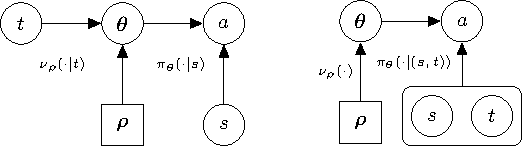
\includegraphics[labellifelong=variationalbound, width=\linewidth]{img/thesis_plots_chapter_lifelong.pdf}
    \caption{\textbf{左图：} 方差上界的几种方法的尺度参数演变。注意 \textit{两步 $\Psi$ 优先} 和 \textit{均匀 $\Psi$} 的 A 值是混叠的。\\
    \textbf{右图：} 方差的变分上界在几种方法下的演变。这里同样，\textit{两步 $\Psi$ 优先} 和 \textit{均匀 $\Psi$} 的对数上界是混叠的。}
    ``CO'' 表示凸优化（convex optimisation）。
    \label{fig:bandit_variational_bound}
\end{figure}


\subsection{实验细节}

\subsubsection{数据集}
\label{subsubsec:datasets_lifelong}
此处提供交易（Trading）和大坝（Dam）任务中涉及过程的更多细节。
对于大坝任务，三种平均入流如 \Cref{fig:dam_inflows} 所示。
还提供了该环境中计算总成本的权重。
对于洪水和未满足需求，第一个入流分布的成本分别为 0.3 和 0.7；第二个入流分布为 0.8 和 0.2；第三个入流分布为 0.35 和 0.65。
对于交易任务，EUR-USD 货币对的历史值见 \Cref{fig:eurusd_dataset}。


\begin{figure*}[t]
  \centering
  \begin{subfigure}{.29\textwidth}
  \centering
  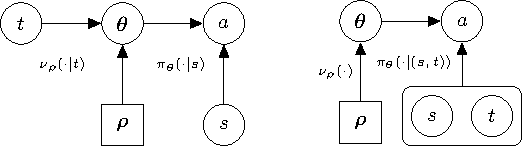
\includegraphics[labellifelong=inflowdam,width=1.3\linewidth]{img/thesis_plots_chapter_lifelong.pdf}
    \end{subfigure}%
  \caption{大坝实验考虑的三种入流分布。}
  \label{fig:dam_inflows}
\end{figure*}


\begin{figure*}[t]
\centering
\begin{subfigure}{.29\textwidth}
  \centering
  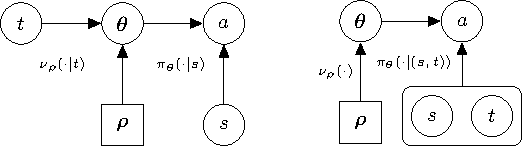
\includegraphics[labellifelong=forexseed0,width=1.3\linewidth]{img/thesis_plots_chapter_lifelong.pdf}
          \caption*{数据集 2009-2012。}
\end{subfigure}%
\hfill
\begin{subfigure}{.29\textwidth}
  \centering
  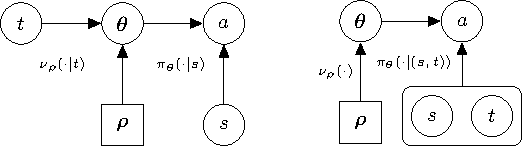
\includegraphics[labellifelong=forexseed1,width=1.3\linewidth]{img/thesis_plots_chapter_lifelong.pdf}
          \caption*{数据集 2013-2016。}
\end{subfigure}%
\hfill
\begin{subfigure}{.29\textwidth}
  \centering
  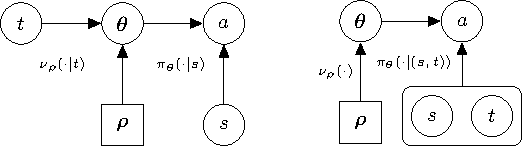
\includegraphics[labellifelong=forexseed2,width=1.3\linewidth]{img/thesis_plots_chapter_lifelong.pdf}
    \caption*{数据集 2017-2020。}
\end{subfigure}%
\captionof{figure}{2009-2020 年间 EUR-USD 货币对的历史汇率，分为三个数据集。}\label{fig:eurusd_dataset}
\end{figure*}
